\documentclass{article}
\usepackage{graphicx} % Required for inserting images
\usepackage{amsmath} 
\newtheorem{lemma}{lemma}
\title{Supplemental Notes on performance Pay}
\author{Jacob Kohlhepp}
\date{\today}

\begin{document}

\maketitle

These notes clarify a few points about the principal-agent models, specifically the effort-based pay and performance pay models.

\section{Timing}

It is helpful to remember the timing of the game is as follows:

\begin{enumerate}
    \item The firm sets the compensation scheme/wage structure by choosing $\alpha, \beta$ (``designing compensation").
    \item Seeing $\alpha, \beta$ the worker decides whether to take the job or the outside option $\bar u$
    \item If they accept the job, the worker chooses effort.
    \item Given effort, output is produced according to $y=e+\epsilon$ and payments occur ($\alpha,\beta$).
\end{enumerate}

Here is a diagram that you may find helpful:

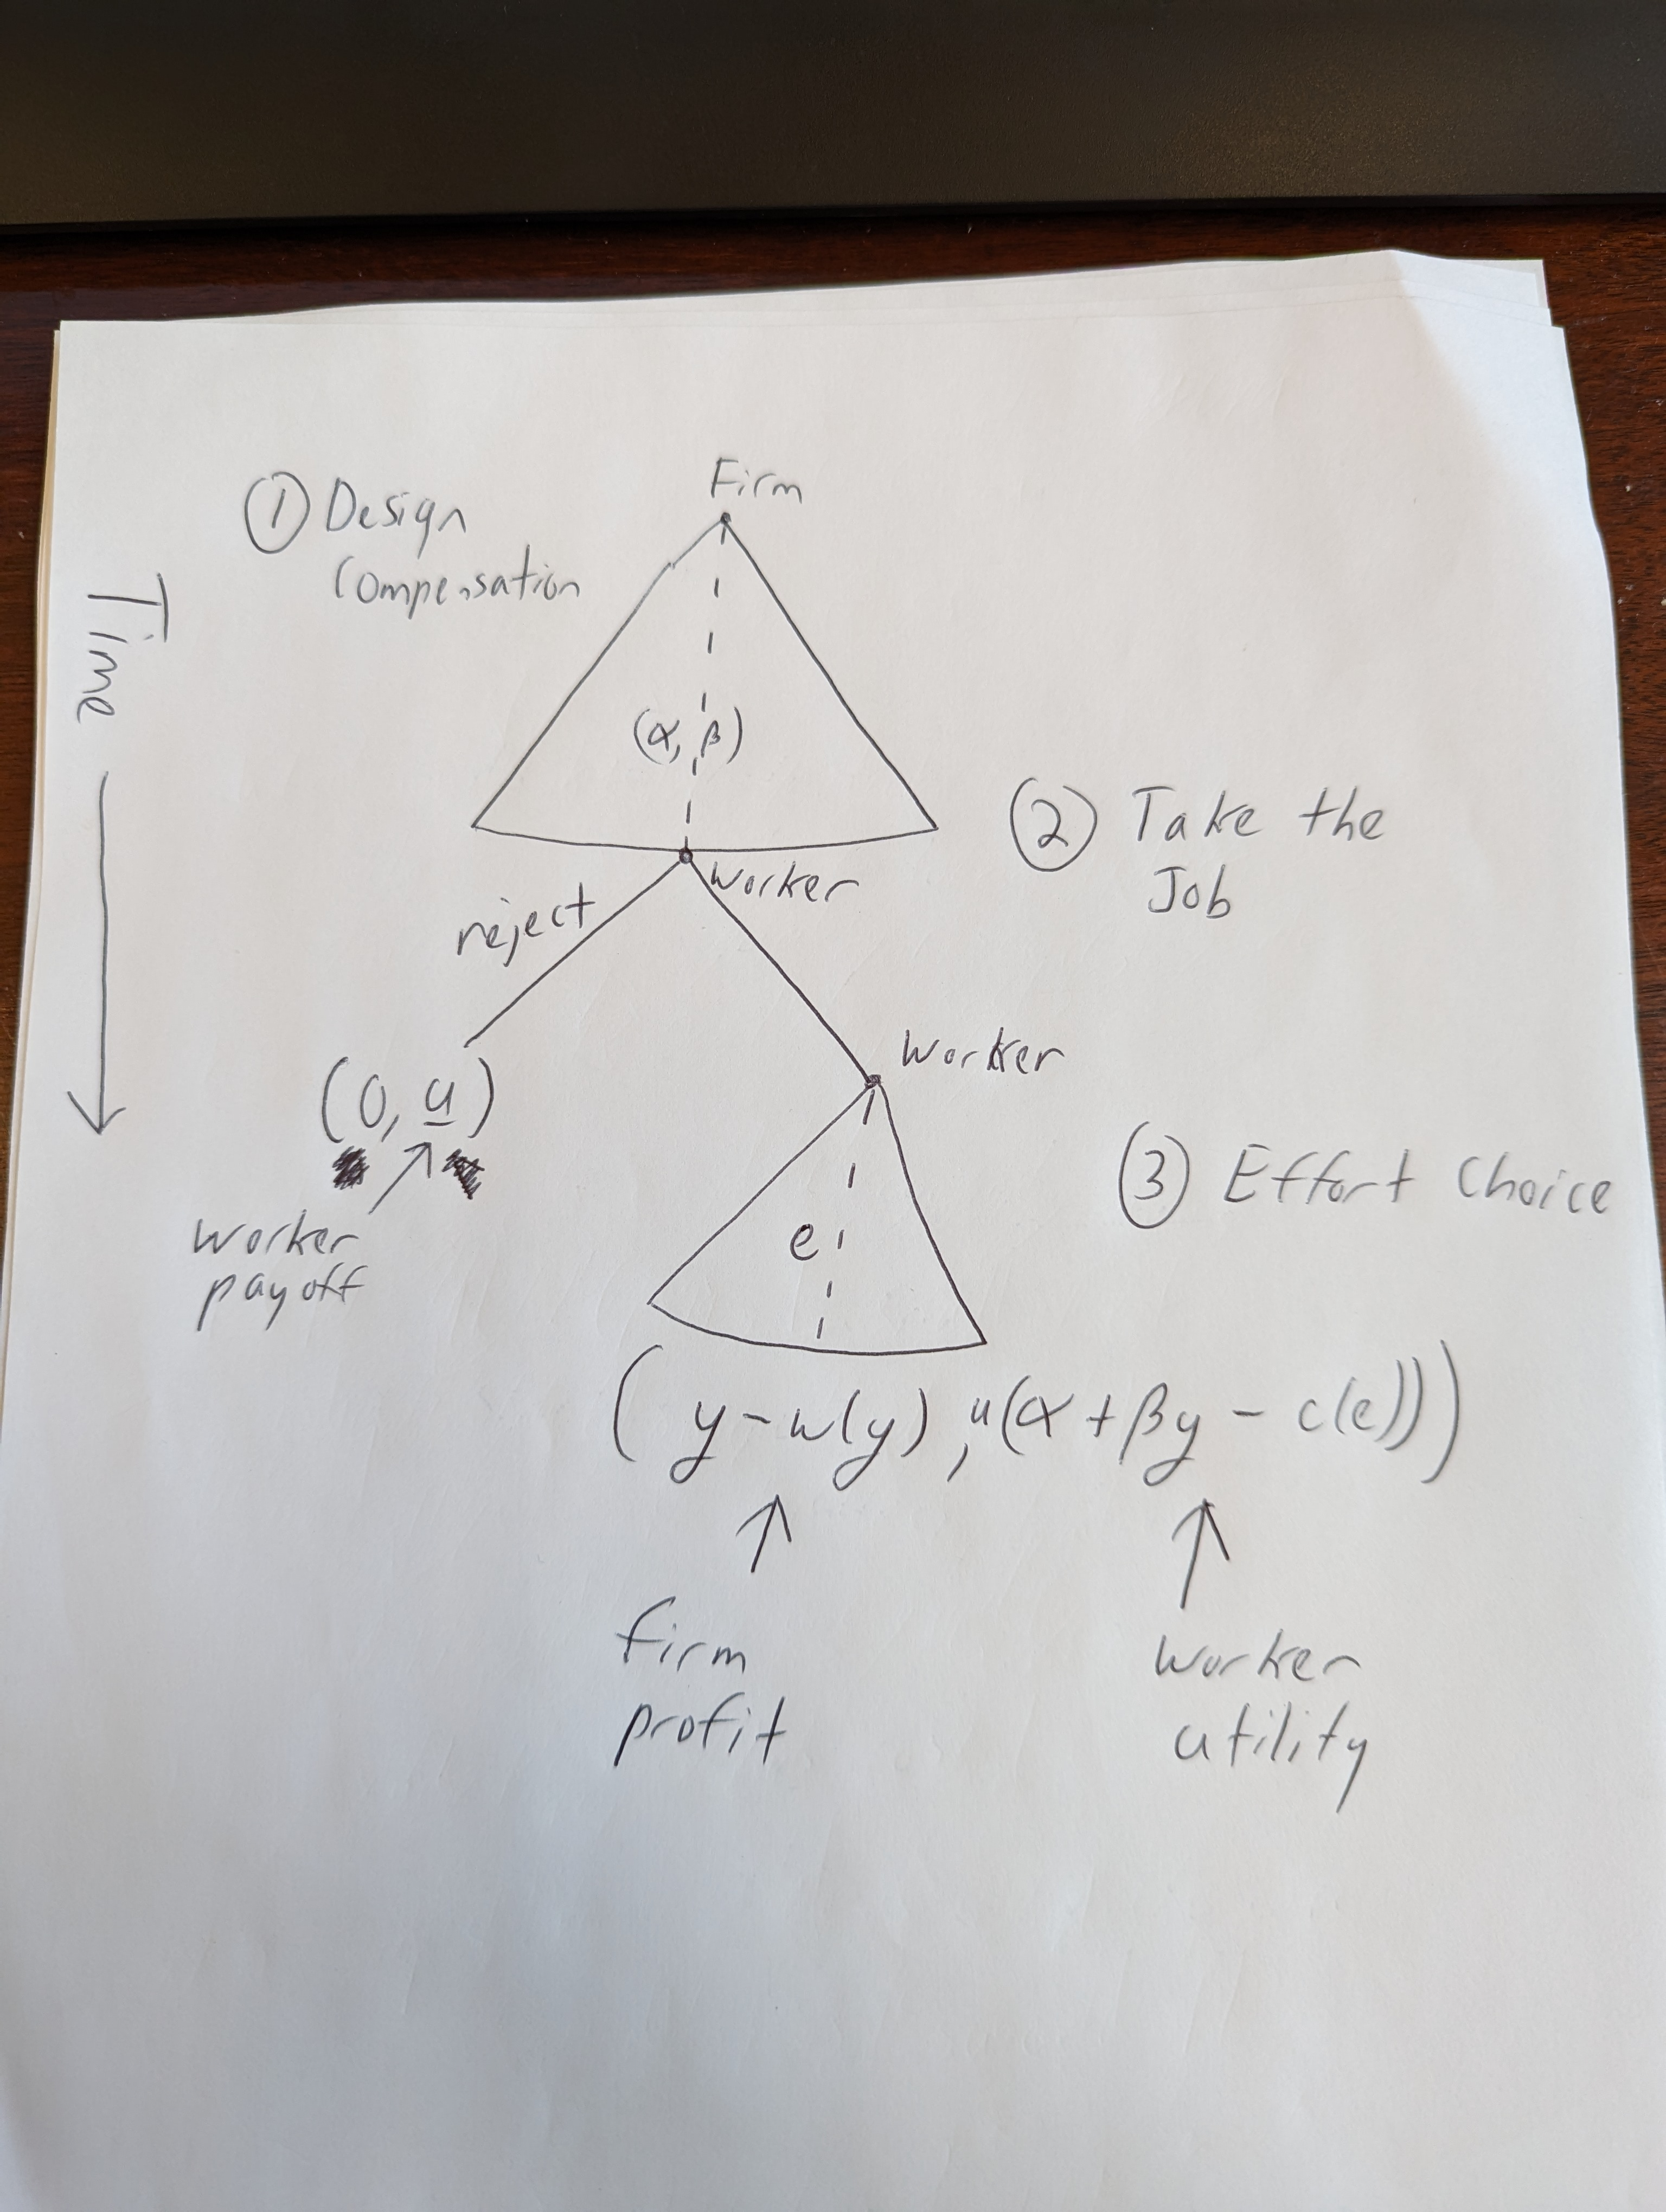
\includegraphics[width=0.7\textwidth]{pictures/PXL_20240131_180348343.jpg}

\section{Certainty Equivalents}

I would like to clarify why we convert things into certainty equivalents. You will not be tested on this, but I think some students will find it helps them understand the big picture. Remember that we assume the worker has exponential utility, which means their expected utility from performance pay $w(y)$ is given by:
\[E [u(w(y))] = \int^{\infty}_{-\infty}  \frac{1-e^{-r w(y)}}{r}f(y)dy\]
where $f$ is the probability density funciton of output.  But this is very complicated, so we want to work with certainty equivalents. My goal is to show you how we get the formula and convince you why we can work using these new units/utility function.

To do this, remember that in our class output is normal. Let $Z \sim N(0,1)$ (a standard normal random variable). Then we can write the wage as $E[w(y)]+ \sqrt{Var(w(y))} \cdot Z$. And we can use this to do the following steps:
\begin{align*}
  E[u(w(y))] &= \int^{\infty}_{-\infty}  \frac{1-e^{-r w(y)}}{r} \frac{e^{-z^2/2}}{\sqrt{2 \pi}} dz\\
              &= 1/r -\int^{\infty}_{-\infty}  \frac{e^{-r w(y)}}{r} \frac{e^{-z^2/2}}{\sqrt{2 \pi}} dz\\
              &= 1/r -\int^{\infty}_{-\infty}  \frac{e^{-r(E[w(y)]+ \sqrt{Var(w(y))}z) }}{r} \frac{e^{-z^2/2}}{\sqrt{2 \pi}} dz\\
            &= 1/r -e^{-r(E[w(y)]}\int^{\infty}_{-\infty}  \frac{e^{-r\sqrt{Var(w(y))}z }}{r} \frac{e^{-z^2/2}}{\sqrt{2 \pi}} dz\\
                     &= 1/r -e^{-r(E[w(y)]}\int^{\infty}_{-\infty}  \frac{e^{-r\sqrt{Var(w(y))}z -z^2/2}}{r\sqrt{2 \pi}} dz\\
\text{Note that: }& -r\sqrt{Var(w(y))}z -z^2/2 = -[2r\sqrt{Var(w(y))}z +\\
& z^2+Var(w(y))r^2]/2 + Var(w(y))r^2/2\\
\text{And further that:}&  = -(z+r\sqrt{Var(w(y))})^2/2  + Var(w(y))r^2/2\\
               &= 1/r -e^{-r(E[w(y)]}\int^{\infty}_{-\infty}  \frac{e^{-(z+r\sqrt{Var(w(y))})^2/2  + Var(w(y))r^2/2}}{r\sqrt{2 \pi}} dz\\
               &= 1/r -e^{-r(E[w(y)]+ Var(w(y))r^2/2}\int^{\infty}_{-\infty}  \frac{e^{-(z+r\sqrt{Var(w(y))})^2/2 }}{r\sqrt{2 \pi}} dz\\
                &= 1/r -1/re^{-r(E[w(y)]+ Var(w(y))r^2/2}\int^{\infty}_{-\infty}  \frac{e^{-(z+r\sqrt{Var(w(y))})^2/2 }}{\sqrt{2 \pi}} dz\\
 \text{the expression inside is a density:}&= 1/r -1/re^{-r(E[w(y)]+ Var(w(y))r^2/2} \cdot 1\\
 &= \frac{1-e^{-r(E[w(y)]+ Var(w(y))r^2/2}}{r} \\
\end{align*}
With this in hand, remember that the certainty equivalent of a wage is the amount of money for sure that makes the worker indifferent betwene the wage and the money. Mathematically this is the $d_w$ that solves:
\[u(d_w) = E [u(w(y))]   \frac{1-e^{-r d_w}}{r}  \]
Plugging in the utility function and the expression we got for $E [u(w(y))] $ this becomes:
\begin{align*}
      \frac{1-e^{-r d_w}}{r} &= \frac{1}{r} \bigg ( 1-e^{-r E[w(y)]+r^2 Var(w(y))/2} \bigg )\\
       1-e^{-r d_w}&=\bigg ( 1-e^{-r E[w(y)]+r^2 Var(w(y))/2} \bigg )\\
       e^{-r d_w}&=e^{-r E[w(y)]+r^2 Var(w(y))/2}\\
        ln(e^{-r d_w})&=ln(e^{-r E[w(y)]+r^2 Var(w(y))/2})\\
        -r d_w&=-r E[w(y)]+r^2 Var(w(y))/2\\
        d_w&= E[w(y)]-\frac{r Var(w(y))}{2}\\
\end{align*}
This is the expression we derived in class! So the certainty equivalent is just a way to re-write the utility in different units (call these CE units). Remember that utility represents preferences (I like wage 1 better than wage 2), and so the units do not usually matter. However it is key that we work all in the same units. This is where I should clarify.

The cost of effort $c(e)$ is already in certainty equivalent units because it is certain! if you don;t believe me, apply the formula: $d_{c(e)} = E[c(e)]-r/2 Var(c(e))$. Because variance is 0, this is just $d_{c(e)}=c(e)$. The same is true for the outside option. We assume that the outside option is $\bar u$ for sure, so by the same argument we have that the certainty equivalent of $\bar u$ is $\bar u$. Putting this together, this means that once we convert the utility from the wage into certainty equivelrnt units using our formula, we can express the worker's expected utility from taking the job as the certainty equivalent of the wage minus the cost of effort (as we have always been doing):
\[ E[w(y)]-\frac{r Var(w(y))}{2} -c(e)=\alpha +\beta e - \frac{r\beta^2 \sigma^2}{2}-c(e)\]
We can also compare this expression to $\bar u$ because both are in CE units. So the following inequality (from step 2 take the job) is valid:
\[E[w(y)]-\frac{r Var(w(y))}{2} -c(e) =\alpha +\beta e - \frac{r\beta^2 \sigma^2}{2}-c(e)\geq  \bar u\]


\section{Effort is Known But Not Contractible}

When we solved the effort-based pay model, we argued that it was more of a benchmark. We argued that effort is not observable and also not measurable, so paying a wage based on effort is not realistic. We then said that is why firms use performance pay, where the wage is based on output ($y$) which tends to be easier to measure and observe. Yet there is a tension in this argument. To see the tension, consider when we solved the performance pay model. In step 3 "Choosing Effort" we get the following condition:
\[\beta = c'(e)\]
In words, the marginal benefit of effort for the worker is equal to the marginal cost. Now, the firm knows the bonus $\beta$ because it chooses $\beta$. And we assumed implicitly that it knows the cost of effort $c(e)$ (otherwise we could not plug this equation into profit in step 1 "Designing Compensation"). But if it knows $c(e)$ and it knows $\beta$, then this implies it knows effort! Further, because $y$ is known, the firm can subtract $e$ from $y$ so it also knows luck/randomness $\epsilon$.

And therein lies the tension: effort-based pay is always better than performance pay, and the firm knows effort, so why cannot the firm use effort pay? The answer is that the firm uses equilibrium logic where it ``puts itself in the shoes of the worker" to determine $e$. So while effort is known to the firm, and the firm can act on this knowledge, it cannot be written into a contract. Meaning in a court of law, the firm cannot prove that the worker exerted a certain amount of effort.

We then say that effort is known but not contractible. In our model of performance pay, this is an implicit and key assumption. And in some sense it is reasonable: the firm may understand that the worker worked hard or slacked off, but may be unable to prove this to the standard of proof required by a court. As a result, it cannot write this into a contract. We will explore this idea more when we think about relational contracts: I cannot prove you slacked off, but I do not need to prove it to terminate you (or not promote you) because these are actions I am taking not contracts.






\end{document}